\section{Angle-scanned phase-encoded 3D imaging}
\label{sec:imaging}

\begin{figure*}[t]
\centering
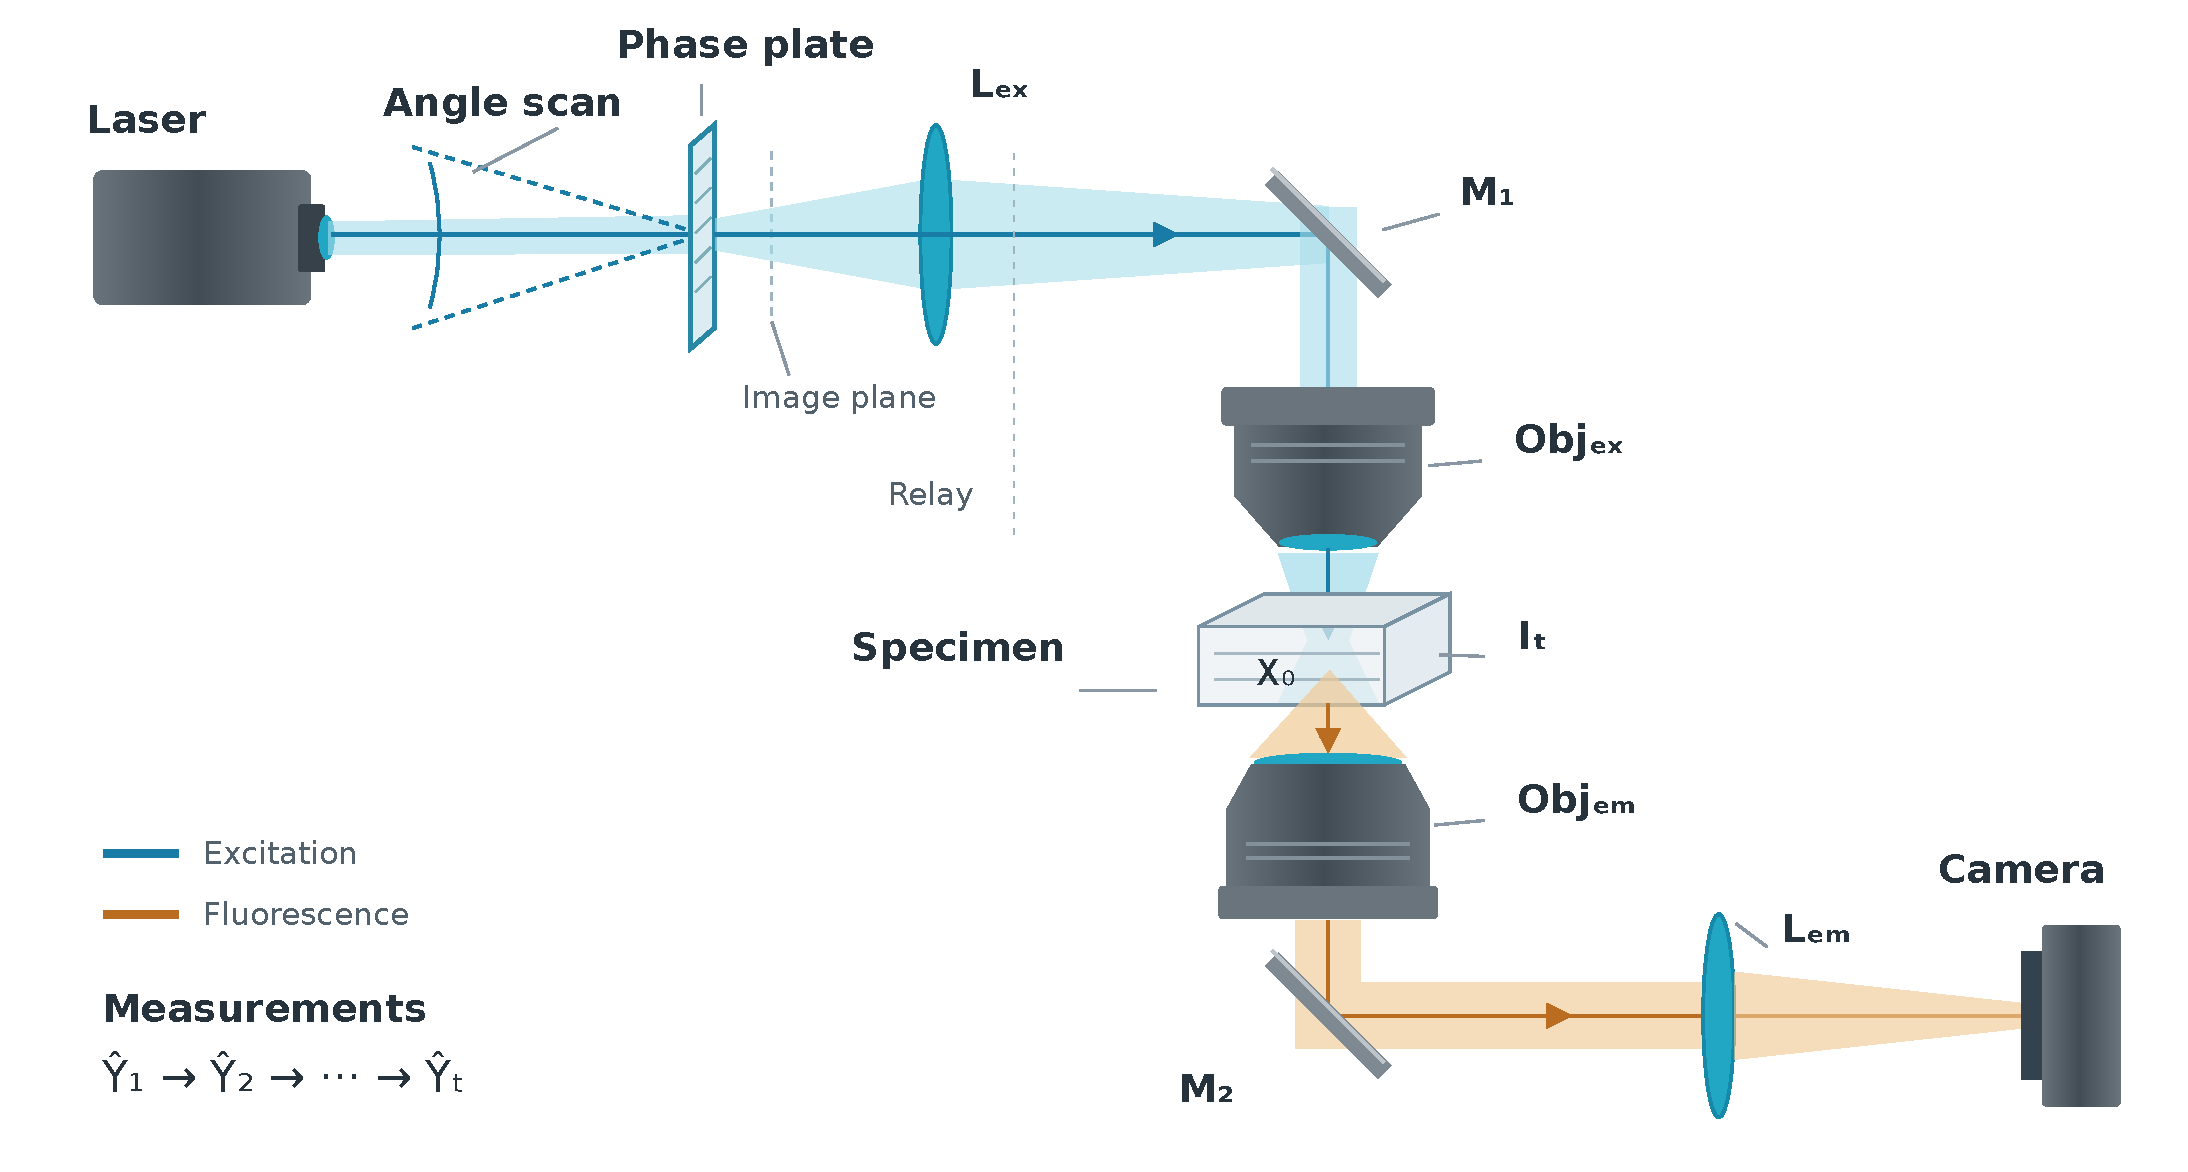
\includegraphics[width=0.585\linewidth]{acquisition.pdf}\hfill
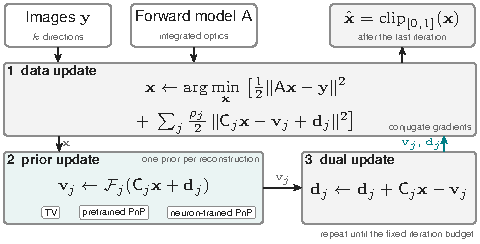
\includegraphics[width=0.40\linewidth]{reconstruction.pdf}
\caption{\textbf{Fixed-focus acquisition and reconstruction.} Left: a tilted plane wave illuminates a fixed phase plate placed $6.6\um$ (specimen-space units) before an intermediate illumination image plane; an NA-0.8 vectorial relay maps the field into the specimen; a camera at a fixed detection focus records one image per illumination angle. Only the input angle changes: plate, specimen and focus are stationary, and nothing is scanned axially. Blue: excitation; orange: fluorescence. Right: multi-slice plug-and-play recovery alternates a conjugate-gradient data-consistency step with one pretrained 2D denoiser applied to the $xy$, $yz$ and $zx$ slices of a shared volume and an $\ell_1$ shrinkage, fused by ADMM.}
\label{fig:system}
\end{figure*}

\paragraph{Acquisition.}
Let $\mathbf r=(x,y)$ and $t$ index the illumination direction. A plane wave $u^{\mathrm{in}}_t(\mathbf r)=a_te^{\mathrm ik_{\mathrm{ex}}\mathbf s_t\cdot\mathbf r}$ with transverse direction $\mathbf s_t=\cos\theta_t(\cos\alpha_t,\sin\alpha_t)$ passes a fixed phase-only plate $\tau(\mathbf r)=e^{\mathrm i\phi(\mathbf r)}$ (\cref{fig:system}). We scan 16 azimuths and 16 signed elevations, $0.5\le\|\mathbf s_t\|\le\sqrt3/2$, so the two scan coordinates set the direction and magnitude of a linear phase gradient across the plate. Angular-spectrum propagation carries $\tau u^{\mathrm{in}}_t$ over the plate-to-image-plane distance $D$; the objective pupil band-limits it to $\mathrm{NA}=0.8$, and a vectorial Richards--Wolf relay \cite{richards1959,marian2007} gives the excitation intensity $I_t(\mathbf r,z)=\sum_{c\in\{x,y,z\}}|E_{t,c}(\mathbf r,z)|^2$ in the specimen. The camera records one planar image per direction; acquisition is therefore fixed-focus but sequential (256 frames for the full scan), not single-shot.

\paragraph{Why the angle encodes depth.}
Three properties of this arrangement matter. (i) \emph{Without the plate}, a tilted plane wave that overfills the field has laterally uniform intensity at every depth, so changing the angle changes nothing in the specimen except, beyond the pupil, whether light arrives at all: the scan alone carries no depth information. (ii) \emph{With the plate in an image plane}, a phase-only screen would give uniform intensity at focus and patterns symmetric about it. Placing the plate a distance $D$ \emph{before} the image plane makes the excitation a 3D speckle-like intensity whose planes differ and whose structure is not mirror-symmetric about focus. (iii) \emph{Tilting the input} multiplies the field after a thin screen by the same linear phase, so the diffracted pattern at a further propagation distance $D+z$ is translated by approximately $(D+z)\,\Delta\mathbf s/\sqrt{1-s^2}$ (the angular memory effect of a thin screen together with the Fresnel shift theorem). Different depths therefore translate at different rates as the angle changes, and every depth receives its own sequence of excitation values. We measure this shear in \cref{sec:res:optics}; it holds at 0.7--0.9 of this rate, with partial decorrelation between angles. By contrast, an amplitude pattern imaged in focus (as with a digital micromirror device) is real-valued at the focal plane, so its defocused intensities are equal at $\pm\Delta z$ and mirror depths are confounded.

\paragraph{Image formation.}
With fluorescence $X_0$, emission PSF $\mathrm{emPSF}$ and pixel region $D_p$, linear unsaturated fluorescence gives
\begin{equation}
Y_t=\mathrm{emPSF}*_3(X_0I_t),\qquad
\hat Y^0_{t,p}=\tfrac{1}{|D_p|}\!\int_{D_p}\!Y_t(\mathbf r,z_{\mathrm{focal}})\,\mathrm d\mathbf r .
\label{eq:forward}
\end{equation}
The product $X_0I_t$ mixes specimen and illumination spatial frequencies before the low-NA blur and pixel averaging, so the detector need not resolve the illumination pattern; depth separation comes from how the excitation sequence varies across depths and angles.

\paragraph{Voxel-integrated operator.}
Optical simulation needs a fine grid ($0.08\um$ optical, $0.32\um$ analysis), reconstruction a coarse one ($0.64\um$). We keep the fine-grid measurement process $\bB$ and let each reconstruction voxel represent constant fluorescence over a $2\times2\times2$ analysis patch, with replication $\bU$ and averaging $\bR$:
\begin{equation}
\bA=\bB\bU,\qquad \bx_{\mathrm{gt}}=\bR\bx_f,\qquad \by=\bB\bx_f+\boldsymbol\varepsilon .
\label{eq:patch}
\end{equation}
Measurements are always generated from the finer object $\bx_f$, so the residual $\boldsymbol\delta_{\mathrm{disc}}=\bB(\bx_f-\bU\bR\bx_f)$ that the basis cannot represent is present in every experiment. Building $\bA$ column by column would need one volumetric simulation per voxel and pattern. Because fluorescence is linear and incoherent, the response to an impulse at fine position $\mathbf r_i$ factorises into the excitation there and a pattern-independent emission footprint, $(\bB_t\delta_i)_p=I_t(\mathbf r_i)\,g_p(\mathbf r_i)$, where $g_p$ is the pooled detector image of an emitter at $\mathbf r_i$ (computed once), so that
\begin{equation}
\bA_{(t,p),j}=\textstyle\sum_{i\in\mathcal P_j} I_t(\mathbf r_i)\,g_p(\mathbf r_i).
\label{eq:factor}
\end{equation}
The factorisation itself follows from linear fluorescence physics; our contribution is to use it to integrate a fine-grid vectorial model exactly over the reconstruction basis at a cost of $O(TPF)$ for $T$ patterns, $P$ detector samples and $F$ fine voxels, instead of $O(TNF\log F)$ for column simulation. The full $36{,}864\times36{,}864$ operator builds in about $110$\,s on one GPU and matches the live forward model to $8\times10^{-7}$ relative error (tolerance $10^{-5}$).

\paragraph{Reconstruction.}
We combine measurement consistency with a pretrained 2D DnCNN \cite{zhang2017} applied to the $xy$, $yz$ and $zx$ slice sets of one shared volume, $\mathcal D_o=\mathsf P_o^{-1}\mathcal D\mathsf P_o$, following plug-and-play priors and multi-slice fusion \cite{venkatakrishnan2013,majee2021}. With one auxiliary volume $\mathbf v_j$, dual $\mathbf d_j$ and penalty $\rho_j$ per branch $j\in\{xy,yz,zx,\mathrm{sp}\}$, ADMM alternates
\begin{align}
\bx^{k+1}&=\arg\min_{\bx}\tfrac12\|\bA\bx-\by\|_2^2+\textstyle\sum_j\tfrac{\rho_j}{2}\|\bx-\mathbf v_j^k+\mathbf d_j^k\|_2^2,\label{eq:admm}\\
\mathbf v_o^{k+1}&=\mathcal D_o(\bx^{k+1}+\mathbf d_o^k),\quad
\mathbf v_{\mathrm{sp}}^{k+1}=\mathcal S_{\lambda/\rho_{\mathrm{sp}}}(\bx^{k+1}+\mathbf d_{\mathrm{sp}}^k),\nonumber
\end{align}
with $\mathbf d_j^{k+1}=\mathbf d_j^k+\bx^{k+1}-\mathbf v_j^{k+1}$, a conjugate-gradient solve of \cref{eq:admm}, soft thresholding $\mathcal S$, back-projection initialisation and a final clip to $[0,1]$. As a non-learned solver we also compute $\arg\min_{0\le\bx\le1}\tfrac12\|\bA\bx-\by\|_2^2+\lambda\,\mathrm{TV}(\bx)$ with isotropic 3D total variation \cite{rudin1992} (ADMM \cite{boyd2011}, 300 iterations). No network is trained for the task; neither solver is a contribution.
